\documentclass[10pt,a4paper,onecolumn]{article}
% \usepackage[utf8]{inputenc}
\usepackage{marginnote}
\usepackage{graphicx}
\usepackage{xcolor}
\usepackage{authblk,etoolbox}
\usepackage{titlesec}
\usepackage{calc}
\usepackage{hyperref}
\hypersetup{breaklinks=true,
            bookmarks=true,
            pdfauthor=
{
      Georgios Detorakis,
  },
            pdftitle=
{
[Re] Multiple dynamical modes of thalamic relay neurons: rhythmic bursting
        and intermittent phase-locking
},
            colorlinks=true,
            citecolor=blue,
            urlcolor=blue,
            linkcolor=blue,
            pdfborder={0 0 0}}
\urlstyle{same}
\usepackage{tcolorbox}
\usepackage{ragged2e}
\usepackage{fontspec}
\usepackage{fontawesome}
\usepackage{caption}
\usepackage{listings}
\usepackage{float,lscape}
\usepackage{xcolor,colortbl}
\usepackage{amssymb,amsmath,array,amsthm}
\usepackage{marvosym}
\usepackage{array}

\makeatletter
\newcommand{\thickhline}{%
    \noalign {\ifnum 0=`}\fi \hrule height 1pt
    \futurelet \reserved@a \@xhline
}
\newcolumntype{"}{@{\hskip\tabcolsep\vrule width 1pt\hskip\tabcolsep}}
\makeatother

\definecolor{Gray}{gray}{0.75}
\definecolor{LightGray}{gray}{0.95}
\lstnewenvironment{code}{\lstset{language=Haskell,basicstyle=\small\ttfamily}}{}



%\usepackage{fancyvrb}
%\VerbatimFootnotes
%\usepackage{graphicx}
%\usepackage{mdframed}
%\newmdenv[backgroundcolor=lightgray]{Shaded}


\usepackage{longtable,booktabs}

\usepackage[
  backend=biber,
%  style=alphabetic,
%  citestyle=numeric
]{biblatex}
\bibliography{detorakis-2016.bib}



% --- Macros ------------------------------------------------------------------
\renewcommand*{\bibfont}{\small \sffamily}

\definecolor{red}{HTML}{CF232B}
\newcommand{\ReScience}{Re{\bfseries \textcolor{red}{Science}}}

\newtcolorbox{rebox}
   {colback=blue!5!white, colframe=blue!40!white,
     boxrule=0.5pt, arc=2pt, fonttitle=\sffamily\scshape\bfseries,
     left=6pt, right=20pt, top=6pt, bottom=6pt}

\newtcolorbox{repobox}
   {colback=red, colframe=red!75!black,
     boxrule=0.5pt, arc=2pt, left=6pt, right=6pt, top=3pt, bottom=3pt}

% fix for pandoc 1.14     
\newcommand{\tightlist}{%
  \setlength{\itemsep}{1pt}\setlength{\parskip}{0pt}\setlength{\parsep}{0pt}}

% --- Style -------------------------------------------------------------------
\renewcommand*{\bibfont}{\small \sffamily}
\renewcommand{\captionfont}{\small\sffamily}
\renewcommand{\captionlabelfont}{\bfseries}

\makeatletter
\renewcommand\@biblabel[1]{{\bf #1.}}
\makeatother

% --- Page layout -------------------------------------------------------------
\usepackage[top=3.5cm, bottom=3cm, right=1.5cm, left=1.5cm,
            headheight=2.2cm, reversemp, includemp, marginparwidth=4.5cm]{geometry}

% --- Section/SubSection/SubSubSection ----------------------------------------
\titleformat{\section}
  {\normalfont\sffamily\Large\bfseries}
  {}{0pt}{}
\titleformat{\subsection}
  {\normalfont\sffamily\large\bfseries}
  {}{0pt}{}
\titleformat{\subsubsection}
  {\normalfont\sffamily\bfseries}
  {}{0pt}{}
\titleformat*{\paragraph}
  {\sffamily\normalsize}


% --- Header / Footer ---------------------------------------------------------
\usepackage{fancyhdr}
\pagestyle{fancy}
%\renewcommand{\headrulewidth}{0.50pt}
\renewcommand{\headrulewidth}{0pt}
\fancyhead[L]{\hspace{-1cm}
\includegraphics[width=4.0cm]{rescience-logo.pdf}}
\fancyhead[C]{}
\fancyhead[R]{} 
\renewcommand{\footrulewidth}{0.25pt}

\fancyfoot[L]{\hypersetup{urlcolor=red}
              \sffamily \ReScience~$\vert$
              \href{http://rescience.github.io}{rescience.github.io}
              \hypersetup{urlcolor=blue}}
\fancyfoot[C]{\sffamily \thepage}
\fancyfoot[R]{\sffamily Sep 2015 $\vert$
                        Volume \textbf{1} $\vert$
                        Issue \textbf{1}}
\pagestyle{fancy}
\makeatletter
\let\ps@plain\ps@fancy
\fancyheadoffset[L]{4.5cm}
\fancyfootoffset[L]{4.5cm}

% --- Title / Authors ---------------------------------------------------------
% patch \maketitle so that it doesn't center
\patchcmd{\@maketitle}{center}{flushleft}{}{}
\patchcmd{\@maketitle}{center}{flushleft}{}{}
% patch \maketitle so that the font size for the title is normal
\patchcmd{\@maketitle}{\LARGE}{\LARGE\sffamily}{}{}
% patch the patch by authblk so that the author block is flush left
\def\maketitle{{%
  \renewenvironment{tabular}[2][]
    {\begin{flushleft}}
    {\end{flushleft}}
  \AB@maketitle}}
\makeatletter
\renewcommand\AB@affilsepx{ \protect\Affilfont}
%\renewcommand\AB@affilnote[1]{{\bfseries #1}\hspace{2pt}}
\renewcommand\AB@affilnote[1]{{\bfseries #1}\hspace{3pt}}
\makeatother
\renewcommand\Authfont{\sffamily\bfseries}
\renewcommand\Affilfont{\sffamily\small\mdseries}
\setlength{\affilsep}{1em}

\LetLtxMacro{\OldIncludegraphics}{\includegraphics}
\renewcommand{\includegraphics}[2][]{\OldIncludegraphics[width=12cm, #1]{#2}}


% --- Document ----------------------------------------------------------------
\title{[Re] Multiple dynamical modes of thalamic relay neurons: 
        rhythmic bursting and intermittent phase-locking}

    \usepackage{authblk}
                        \author[1]{Georgios Detorakis}
                        \affil[1]{ Department of Cognitive Sciences, UC Irvine, CA, USA}
            
\date{\vspace{-5mm}
    \sffamily \small \href{mailto:gdetorak@uci.edu}{gdetorak@uci.edu}}


\setlength\LTleft{0pt}
\setlength\LTright{0pt}


\begin{document}
\maketitle

\marginpar{
  %\hrule
  \sffamily\small
  %\vspace{2mm}
  {\bfseries Editor}\\
  Name Surname\\

  {\bfseries Reviewers}\\
        Name Surname\\
        Name Surname\\
  
  {\bfseries Received}  Sep, 1, 2015\\
  {\bfseries Accepted}  Sep, 1, 2015\\
  {\bfseries Published} Sep, 1, 2015\\

  {\bfseries Licence}   \href{http://creativecommons.org/licenses/by/4.0/}{CC-BY}

  \begin{flushleft}
  {\bfseries Competing Interests:}\\
  The authors have declared that no competing interests exist.
  \end{flushleft}

  \hrule
  \vspace{3mm}

  \hypersetup{urlcolor=white}
  
    \vspace{-1mm}
  \begin{repobox}
    \bfseries\normalsize
      \href{http://github.com/rescience/rescience-submission/article}{\faGithubAlt~Article repository}
  \end{repobox}
      \vspace{-1mm}
  \begin{repobox}
    \bfseries\normalsize
      \href{http://github.com/rescience/rescience-submission/code}{\faGithubAlt~Code repository}
  \end{repobox}
        \hypersetup{urlcolor=blue}
}

\begin{rebox}
\sffamily {\bfseries A reference implementation of}
\small
\begin{flushleft}
\begin{itemize}
    \item[→] \emph{Multiple dynamical modes of thalamic relay neurons: rhythmic
        bursting and intermittent phase-locking}, Wang, X-J, Neuroscience,
        59(1), pg. 21--31, 1994.
  \end{itemize}\par
\end{flushleft}
\end{rebox}


\section{Introduction}\label{introduction}

This work introduces a reference implementation of a neuron model 
for thalamocortical relay neurons, \cite{wang:1994} proposed by X-J Wang.
The model is conductance-based and takes advantage of an interplay between 
a T-type calcium current and a non-specific cation sag current and thus it
is able to generate spindle and delta rhythms. Another feature of this model
is the presence of an intermittent phase-locking phenomenon
where action potentials of sodium take place in a non-periodic manner, despite
the fact that they are phase-locked to the periodic input current. Finally,
the model is capable of generating tonic spike patterns. The reference 
implementation in this work, does not aim to reproduce all the results of 
the original article, but some of them in order to test if the model can be
easily reproduced and at what degree the original results are reproducible.
The source code of reference implementation is written in Python (Numpy,
Scipy, Matplotlib and Scikit-image). 


\section{Methods}\label{methods}

The model is described in this section following the paradigm of 
Nordlie et al, \cite{nordlie:2009}. Therefore, a brief description of
the model, equations, parameters and inputs are given in the form of 
tables. 

Table~\ref{Table:1} provides a description of the model and Table~\ref{Table:2}
gives a glimpse of the input used during simulations. Table~\ref{Table:3}
introduces the equations of the model. The neuron model is conductance-based
consisting in four differential equations describing the dynamics of membrane
potential and the kinetics of a T-Type calcium current, a Sag current channel
and a Potassium channel. The rest currents are described by algebraic
equations. Finally, all simulations parameters are given in
Table~\ref{Table:5} and the simulations times can be found in
Table~\ref{Table:2}.

The reference implementation has been done in a Python class (Python $3.5.1$)
along with Numpy (version $1.10.4$), Scipy (version $0.17.0$) and Matplotlib
($1.5.1$). The numerical integration has been done by the \emph{ode} method 
of Scipy \emph{integrate} package taking advantage of the \emph{dopri5} 
method, which is quite close to the one used by the author of the original 
article (the author has numerically integrated the system of the four ODEs
by using a fifth-order adaptive size Runge-Kutta method). In addition, we 
provide in our implementation the choice of using \emph{BDF} or \emph{Adams}
multistep methods \cite{ascher:1998} (the choice of \emph{BDF} or \emph{Adams}
does not alter the numerical results but it's much faster than \emph{dopri5}).

All the simulations ran on a Dell OptiPlex $7040$, equipped with a sixth
generation i$7$ processor, $8$GB of physical memory and running Arch Linux
as operating system. The total execution time of simulations is $38.76$
seconds and the total consumed memory is $66$MB (if one choose to run 
the code for the parameters diagrams, the total execution time elevates 
to $3$ to $4$ days depending on the machine). Table~\ref{Table:3}, shows
all the parameters we used in order to produce our results (see Results). 
No any other implementation of this model found by the authors in order 
to make any further comparison with.  
%%
\begin{table}[!htbp]
    \centering
    \begin{tabular}{ll}
        \thickhline
        \multicolumn{2}{c}{Model Summary} \\\thickhline
        \rowcolor{Gray}
        Populations  & No population -- one neuron model \\\rowcolor{LightGray}
        Topology     & -- \\ \rowcolor{Gray}
        Connectivity & -- \\ \rowcolor{LightGray}
        Neuron Model & Hodgkin-Huxley conductance-based \\\rowcolor{Gray}
        Channel Models & \\ \rowcolor{LightGray}
        Synapse Model & -- \\ \rowcolor{Gray}
        Plasticity & -- \\ \rowcolor{LightGray}
        Input & Constant current or periodic rectangular pulses \\\rowcolor{Gray}
        Measurements & Membrane potential, channels activation, phase plane \\
        \thickhline
    \end{tabular}
    \caption{{\bfseries \sffamily Summary of the model}} 
    \label{Table:1}
\end{table}
 %%  

%%
\begin{table}[!htbp]
    \centering
    \begin{tabular}{ccc}
        \thickhline
        \multicolumn{3}{c}{Simulation Time} \\ \thickhline
        Figure & Simulation Time ($s$) & Integration Step ($ms$) \\ \rowcolor{LightGray}
        $1$ & $2$, $5\times period$ & $0.05$ \\ \rowcolor{Gray}
        $2$ & $2$ & $0.05$ \\ \rowcolor{LightGray} 
        $3$ & $8$ & $0.05$  \\ \rowcolor{Gray} 
        $4$ & $2.5$ & $0.05$  \\ \rowcolor{LightGray}  
        $5$ & $2$ & $0.05$  \\ \thickhline
    \end{tabular}
    \caption{{\bfseries \sffamily Simulations Time.}}
    \label{Table:2}
\end{table}
%%  

%%
\begin{table}[!htbp]
    \centering
    \begin{tabular}{llcccc}
        \thickhline
        \multicolumn{6}{c}{Input} \\\thickhline
        Figure  & Type & Form & \parbox[t]{1.5cm}{Frequency
            ($\frac{1}{P_0}$,$Hz$)} & 
            \parbox[t]{1.5cm}{Duration ($p$, $ms$)} &
            \parbox[t]{1.5cm}{Amplitude ($\mu A / cm^2$)} \\
        \thickhline \rowcolor{LightGray}
        Figure~$1$ & Periodic & 
            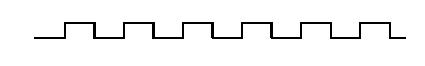
\includegraphics[width=0.1\textwidth]{figs/pulse.pdf} &
            \parbox[t]{1.1cm}{$5$, $10$} &
            \parbox[t]{1.1cm}{$10$, $40$} &
            \parbox[c]{0.3cm}{$-1.0$}
            \\\rowcolor{Gray}
        Figure~$2$ & Constant  & 
        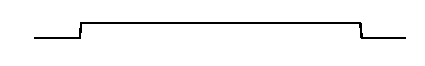
\includegraphics[width=0.1\textwidth]{figs/const.pdf} &
        -- & -- & \parbox[c]{0.3cm}{$+3.0$ \\ $0.0$ $-0.5$ $-0.55$ $-0.6$ $-0.8$
        $-1.3$ $-2.1$} 
        \\\rowcolor{LightGray}
        Figure~$3$ & Constant  & 
            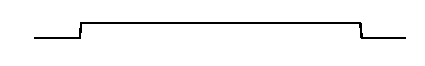
\includegraphics[width=0.1\textwidth]{figs/const.pdf} &
            -- & -- & \parbox[c]{0.3cm}{$-0.95$}
        \\\rowcolor{Gray}
        Figure~$4$ & Constant  & 
            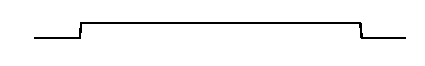
\includegraphics[width=0.1\textwidth]{figs/const.pdf} &
            -- & -- & \parbox[c]{0.3cm}{$[-2,0]$}
        \\\rowcolor{LightGray}
        Figure~$5$ & Constant  & 
            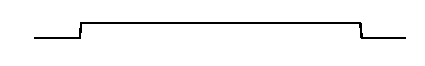
\includegraphics[width=0.1\textwidth]{figs/const.pdf} &
            -- & -- & \parbox[c]{0.3cm}{$[-2,0]$} \\
        \thickhline
    \end{tabular}
    \caption{{\bfseries \sffamily Description of the applied current
        $I_{\text{app}}$ }}
    \label{Table:3}
\end{table}
%%  


\begin{table}[!htbp]
    \centering
    \begin{tabular}{p{1.5cm}ll}
        \thickhline
        \multicolumn{2}{c}{Neuron Model} \\\thickhline
        \rowcolor{Gray}
        Name  &  Thalamocortical relay neuron  \\ \rowcolor{LightGray}
        Type  &  Conductance-based neuron  \\ \rowcolor{Gray}
        Membrane Potential & $
            \begin{aligned}
                C_m \frac{dV(t)}{dt} &= -I_T - I_h - I_{Na}
                  - I_K - I_{Na(P)} - I_L + I_{\text{app}}
              \end{aligned}$ \\ \rowcolor{LightGray}
        T-Type Calcium Current ($I_T$) & $
            \begin{aligned}
                I_T &= g_T \cdot s^3_{\infty}(V)\cdot h \cdot (V-V_{Ca}) \\
                s_{\infty}(V) &= \frac{1}{1 + \exp(-\frac{V+65}{7.8})} \\
                \frac{dh(t)}{dt} &= \phi_h \frac{h_{\infty}(V) - h}{\tau_h(V)} \\
                h_{\infty}(V) &= \frac{1}{1 + \exp(\frac{V-\theta_h}{k_h})} \\
                \tau_h(V) &= h_{\infty}\exp(\frac{V+162.3}{17.8}) + 20
            \end{aligned} $
            \\ \rowcolor{Gray}
        Sag Current ($I_h$) & $
            \begin{aligned}
                I_h &= g_h \cdot H^2 \cdot (V-V_h) \\
                H_{\infty}(V) &= \frac{1}{1 + \exp(\frac{V+69}{7.1})} \\
                \frac{dH(t)}{dt} &= \phi_H \frac{H_{\infty}(V) - H}{\tau_H(V)} 
            \end{aligned} $
            \\ \rowcolor{LightGray} 
        Hodgkin-Huxley Currents ($I_K$) and ($I_{Na}$) & $
            \begin{aligned}
                I_{K} &= g_K \cdot n^4 \cdot (V - V_K) \\
                \frac{dn(t)}{dt} &= \phi_n \frac{n_{\infty}(V) - n(t)}{\tau_n(V)} \\
                n_{\infty}(\sigma_K, V) &= \frac{\alpha_n(\sigma_K, V)}
                        {\alpha_n(\sigma_K, V) + \beta_n(\sigma_K, V)} \\
                \tau_n(\sigma_K, V) &= \frac{1}{\alpha_n(\sigma_K, V)
                        + \beta_n(\sigma_K, V)} \\
                \alpha_n(\sigma_K, V) &= \frac{-0.01 (V + 45.7 - \sigma_K)}
                {\exp(-0.1(V + 45.7 - \sigma_K)) - 1} \\ 
                \beta_n(\sigma_K, V) &= 0.125 \exp(-\frac{V + 55.7 -
                \sigma_K}{80}) \\
                I_{Na} &= g_{Na} \cdot m^3_{\infty}(\sigma_{Na}, V)
                    \cdot (0.85 - n) \cdot (V - V_{Na}) \\
                    m_{\infty}(V) &= \frac{\alpha_m(\sigma_{Na}, V)}
                        {\alpha_m(\sigma_{Na}, V) + \beta_m(\sigma_{Na}, V)} \\
                \alpha_m(\sigma_{Na}, V) &= -0.1 \frac{V + 29.7 - \sigma_{Na}}
                    {\exp(-0.1(V + 54.7 - \sigma{Na})) - 1} \\
                \beta_m(\sigma_{Na}, V) &= 4\exp(-\frac{V+54.7-\sigma_{Na}}{18})
            \end{aligned} $ \\ \rowcolor{Gray} 
        Persistent Sodium Currents ($I_{Na(P)}$) & $
                \begin{aligned}
                    I_{Na(P)} &= g_{Na(P)} \cdot m^3_{\infty}(\sigma_{Na(P)},
                    V) \cdot (V - V_{Na}) \\
                \end{aligned} $
            \\ \rowcolor{LightGray}
        Leak Current ($I_L$) &  $
            \begin{aligned}
                I_L &= g_L \cdot (V - V_L) \\
            \end{aligned} $ \\ \thickhline
    \end{tabular}
    \caption{{\bfseries \sffamily Description of the neuron model}} 
    \label{Table:4}
\end{table}

\begin{landscape}
\begin{table}[!htbp]
    \centering
    \begin{tabular}{p{1.5cm}lllllll}
        \thickhline
        \multicolumn{5}{c}{Model Parameters} \\\thickhline \rowcolor{Gray}
        Currents Type  & Common &  Figure $1$ & Figure $2$ & Figure $3$ &
        Figure $4$  & Figure $5$ \\
        \thickhline \rowcolor{LightGray}
        Membrane Potential & $
            \begin{aligned}
                C_m &= 1 \mu F/cm^2 \\
                V_0 &= -74mV
            \end{aligned} $ & & & \\\rowcolor{Gray}
        T-Type Calcium Current & $
            \begin{aligned}
                \phi_h &= 2 \\
                V_{Ca} &= 120mV
            \end{aligned} $ & $
            \begin{aligned}
                g_T &= 1 mS/cm^2 \\
                \theta_h &= -81 mV \\
                k_h &= 6.25 mV^{-1}
            \end{aligned} $ & $
            \begin{aligned}
                g_T &= 0.3 mS/cm^2\\
                \theta_h &= -79 mV \\
                k_h &= 5 mV^{-1}
            \end{aligned} $ & $
            \begin{aligned}
                g_T &= 0.3 mS/cm^2\\
                \theta_h &= -75 mV \\
                k_h &= 5 mV^{-1}
            \end{aligned} $ & $
            \begin{aligned}
                g_T &= 0.3/0.25/0.2 mS/cm^2\\
                \theta_h &= -81 mV \\
                k_h &= 6.25 mV^{-1}
            \end{aligned} $ & $
            \begin{aligned}
                g_T &= 1.0/0.7 mS/cm^2\\
                \theta_h &= -79 mV \\
                k_h &= 5 mV^{-1}
            \end{aligned} $ 
            \\\rowcolor{LightGray}
        Sag Current & $
            \begin{aligned}
                \phi_H &= 1 \\
                g_h &= 0.04 mS/cm^2 \\
                V_h &= -40 mV
            \end{aligned} $
        & & & \\\rowcolor{Gray}
        Hodgkin-Huxley Currents & $
            \begin{aligned}[l]
                g_K &= 30 mS/cm^2 \\
                V_K &= -80 mV \\
                \phi_n &= 28.5\\
                \sigma_K &= 10 \\
            \end{aligned} 
            \begin{aligned}[r]
                g_{Ca} &= 42 mS/cm^2 \\
                V_{Ca} &= 55 mV \\
            \end{aligned} $
            & $\sigma_{Na} = 3mV$ & $\sigma_{Na} = 6mV$ & $\sigma_{Na} = 6mV$ &
            $\sigma_{Na} = 3mV$ & $\sigma_{Na} = 6mV$
            \\\rowcolor{LightGray}
        Persistent Sodium Currents & $
            \begin{aligned}
                V_{Na(P)} &= 55 mV \\
                \sigma_{Na(P)} &= -5 \\
                g_{Na(P)} = 9 mS / cm^2 
            \end{aligned} $
            & & & & &  
            \\\rowcolor{Gray}
        Leak Current & & $
            \begin{aligned}
                g_L &= 0.1 mS/cm^2\\
                V_L &= -72 mV
            \end{aligned} $ & $
            \begin{aligned}
                g_L &= 0.12 mS/cm^2\\
                V_L &= -70 mV
            \end{aligned} $ & $
            \begin{aligned}
                g_L &= 0.08 mS/cm^2\\
                V_L &= -70 mV
            \end{aligned} $ & $
            \begin{aligned}
                g_L &= 0.08 mS/cm^2\\
                V_L &= -70 mV 
            \end{aligned} $ & $
            \begin{aligned}
                g_L &= 0.12/0.04 mS/cm^2\\
                V_L &= -70 mV 
            \end{aligned} $ \\
        \thickhline
    \end{tabular}
    \caption{{\bfseries \sffamily Simulations Parameters}} 
    \label{Table:5}
\end{table}
\end{landscape}


\section{Results}\label{results}

We simulated the model described in Table~\ref{Table:4} using the parameters
given in Table~\ref{Table:5} and the corresponding input (see
Table~\ref{Table:3} for three different cases). First, we verified 
that the model is able to generate different types of burst responses such
as in figure $1$ of the original article. Thus we applied a periodic 
current pulse of $-1 \mu A/cm^2$ amplitude at several different frequencies
(in the original article frequency is referred as $\frac{1}{P_0}$) ranging
from $0.1Hz$ to $15Hz$ with a resolution (discretization) of $300$ points
(parameters diagram in Figure~\ref{Fig:1} left panel). In addition, we
picked up three specific frequencies ($\frac{1}{P_0}=10, 10, 5$ and pulse
duration $p=10, 40, 40ms$ ($\frac{p}{P_0} = 0.1, 0.4, 0.2$). 
The results are shown in Figure~\ref{Fig:1}, right panels. It is apparent that
the reference implementation can achieve the same behavior as the original
implementation. The parameters correspond to the proper behavior of the model.
%%
\begin{figure}[!htbp]
    \centering
    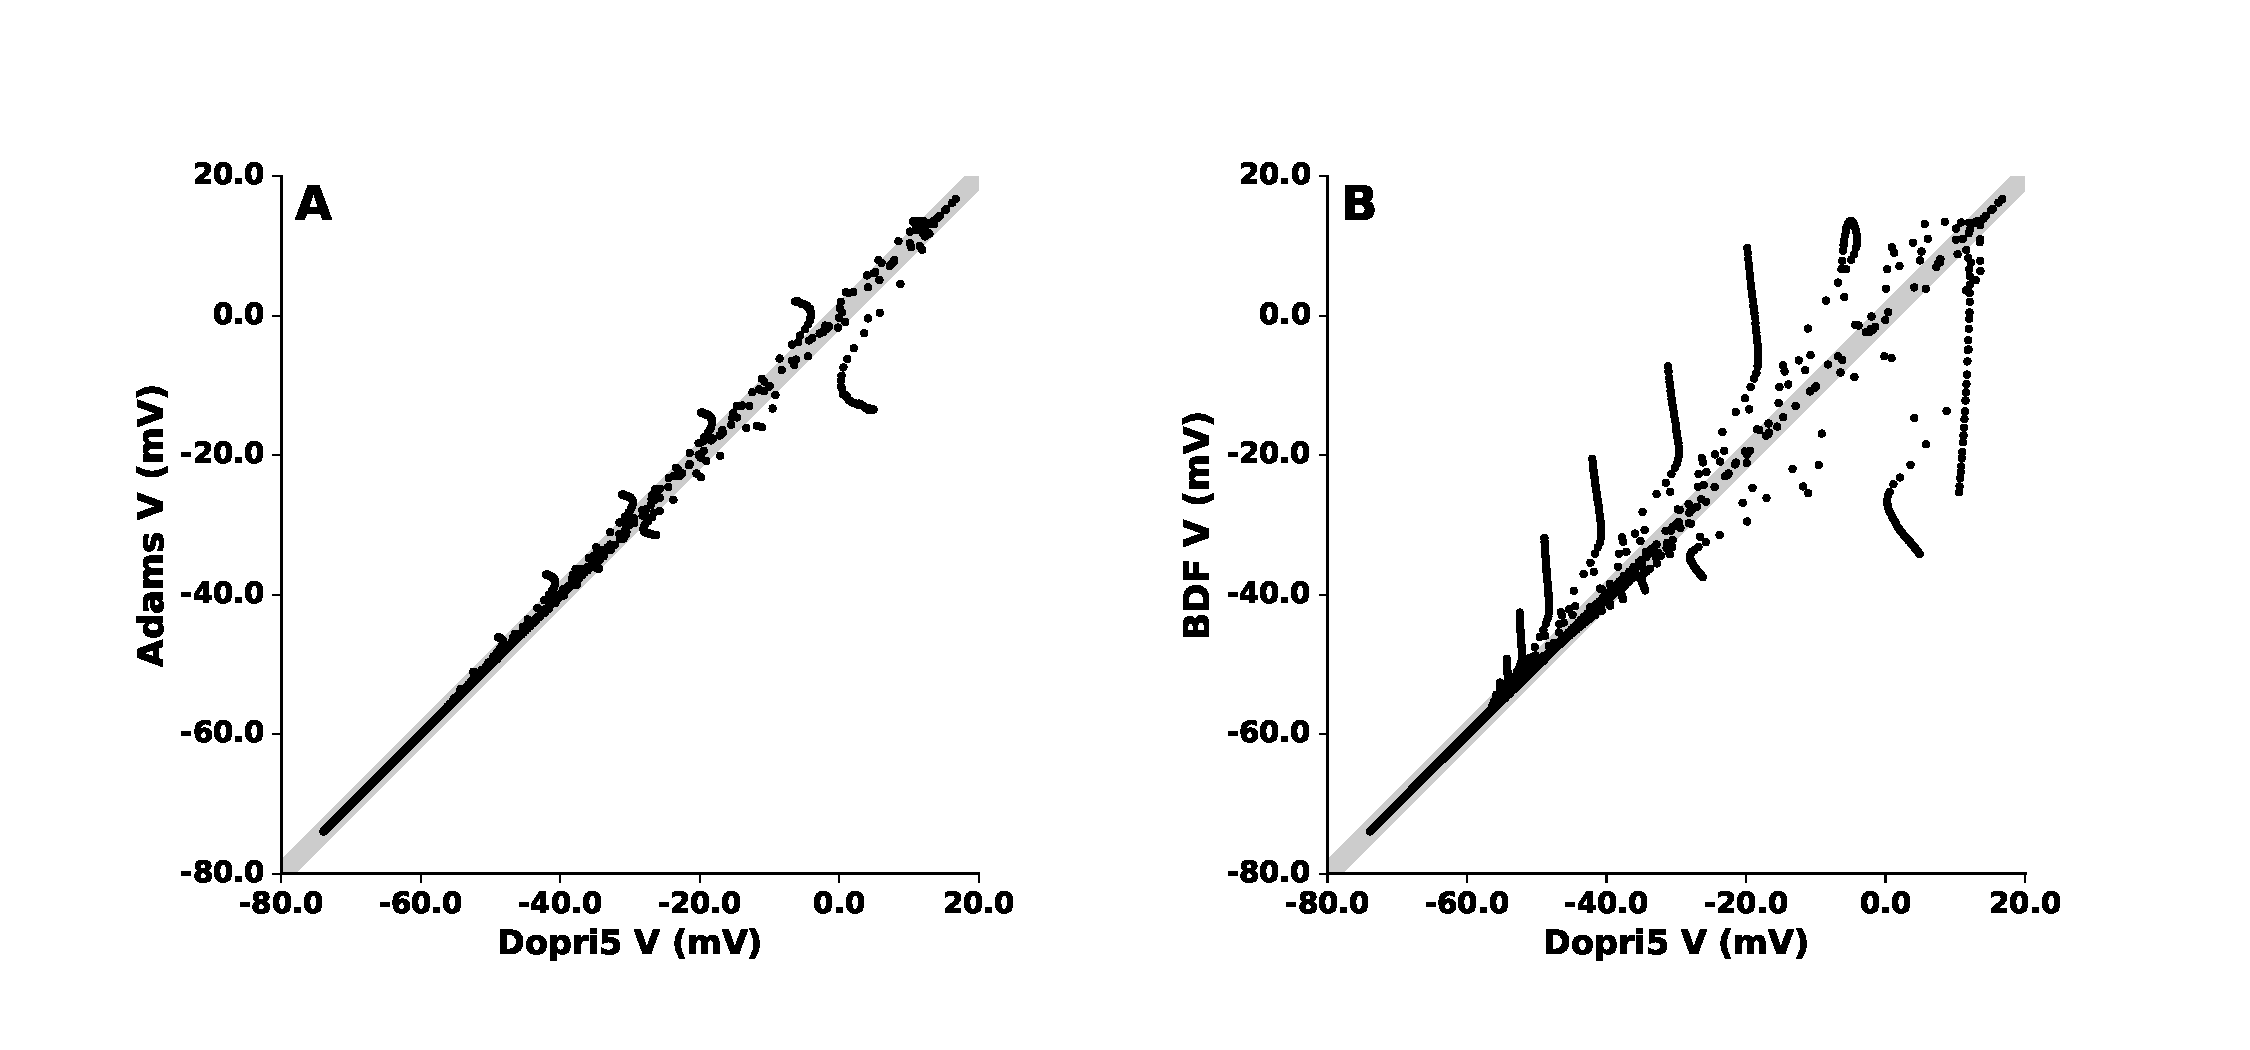
\includegraphics[width=1.0\textwidth]{figs/Figure1.pdf}
    \caption{{\bfseries \sffamily Responses to rhythmic hyperpolarizations.}
        We stimulate the model with a periodic pulse with frequency
        $\frac{1}{P_0}$ and we record the response of the model. All the
        parameters for this simulation are given in Table~\ref{Table:3}. 
        {\bfseries \sffamily Left Panel:} shows a range of frequencies
        $\frac{1}{P_0}$ from $0.1Hz$ to $15Hz$ versus the ratio
        $\frac{p}{P_0}$. 
        {\bfseries \sffamily Right Panels:} 
        {\bfseries \sffamily Red} color demonstrates a case where only
        subthreshold spikes are generated, when the frequency of the periodic
        pulse is $\frac{1}{P_0} = 10 Hz$ and $\frac{p}{P_0} = 0.1$. 
        {\bfseries \sffamily Blue} indicates bursts of one spike, when the
        frequency is $\frac{1}{P_0} = 10Hz$ and $\frac{p}{P_0} = 0.4$.
        {\bfseries \sffamily Black} shows a case of two spikes bursts. Here
        the frequency is $\frac{1}{P_0} = 5 Hz$ and $\frac{p}{P_0} = 0.2$.}
    \label{Fig:1}
\end{figure}
%%

In a second case, we used a steady current varying only its amplitude and 
keeping the rest parameters fixed. Hence, we used $8$ different current
amplitudes ($3, 0, -0.5, -0.55, -0.6, -0.8, -1.3$ and $-2.1 \mu A/cm^2$) and
Figure~\ref{Fig:2} illustrates the results of our simulations, which
correspond to figure $3$ of \cite{wang:1994}. Again original results
are reproducible and the model is capable of generating repetitive firing,
resting state, subthreshold oscillation, $10 Hz$ bursting, $3Hz$ bursting
and hyperpolarized steady activity. 
%%
\begin{figure}[!htbp]
    \centering
    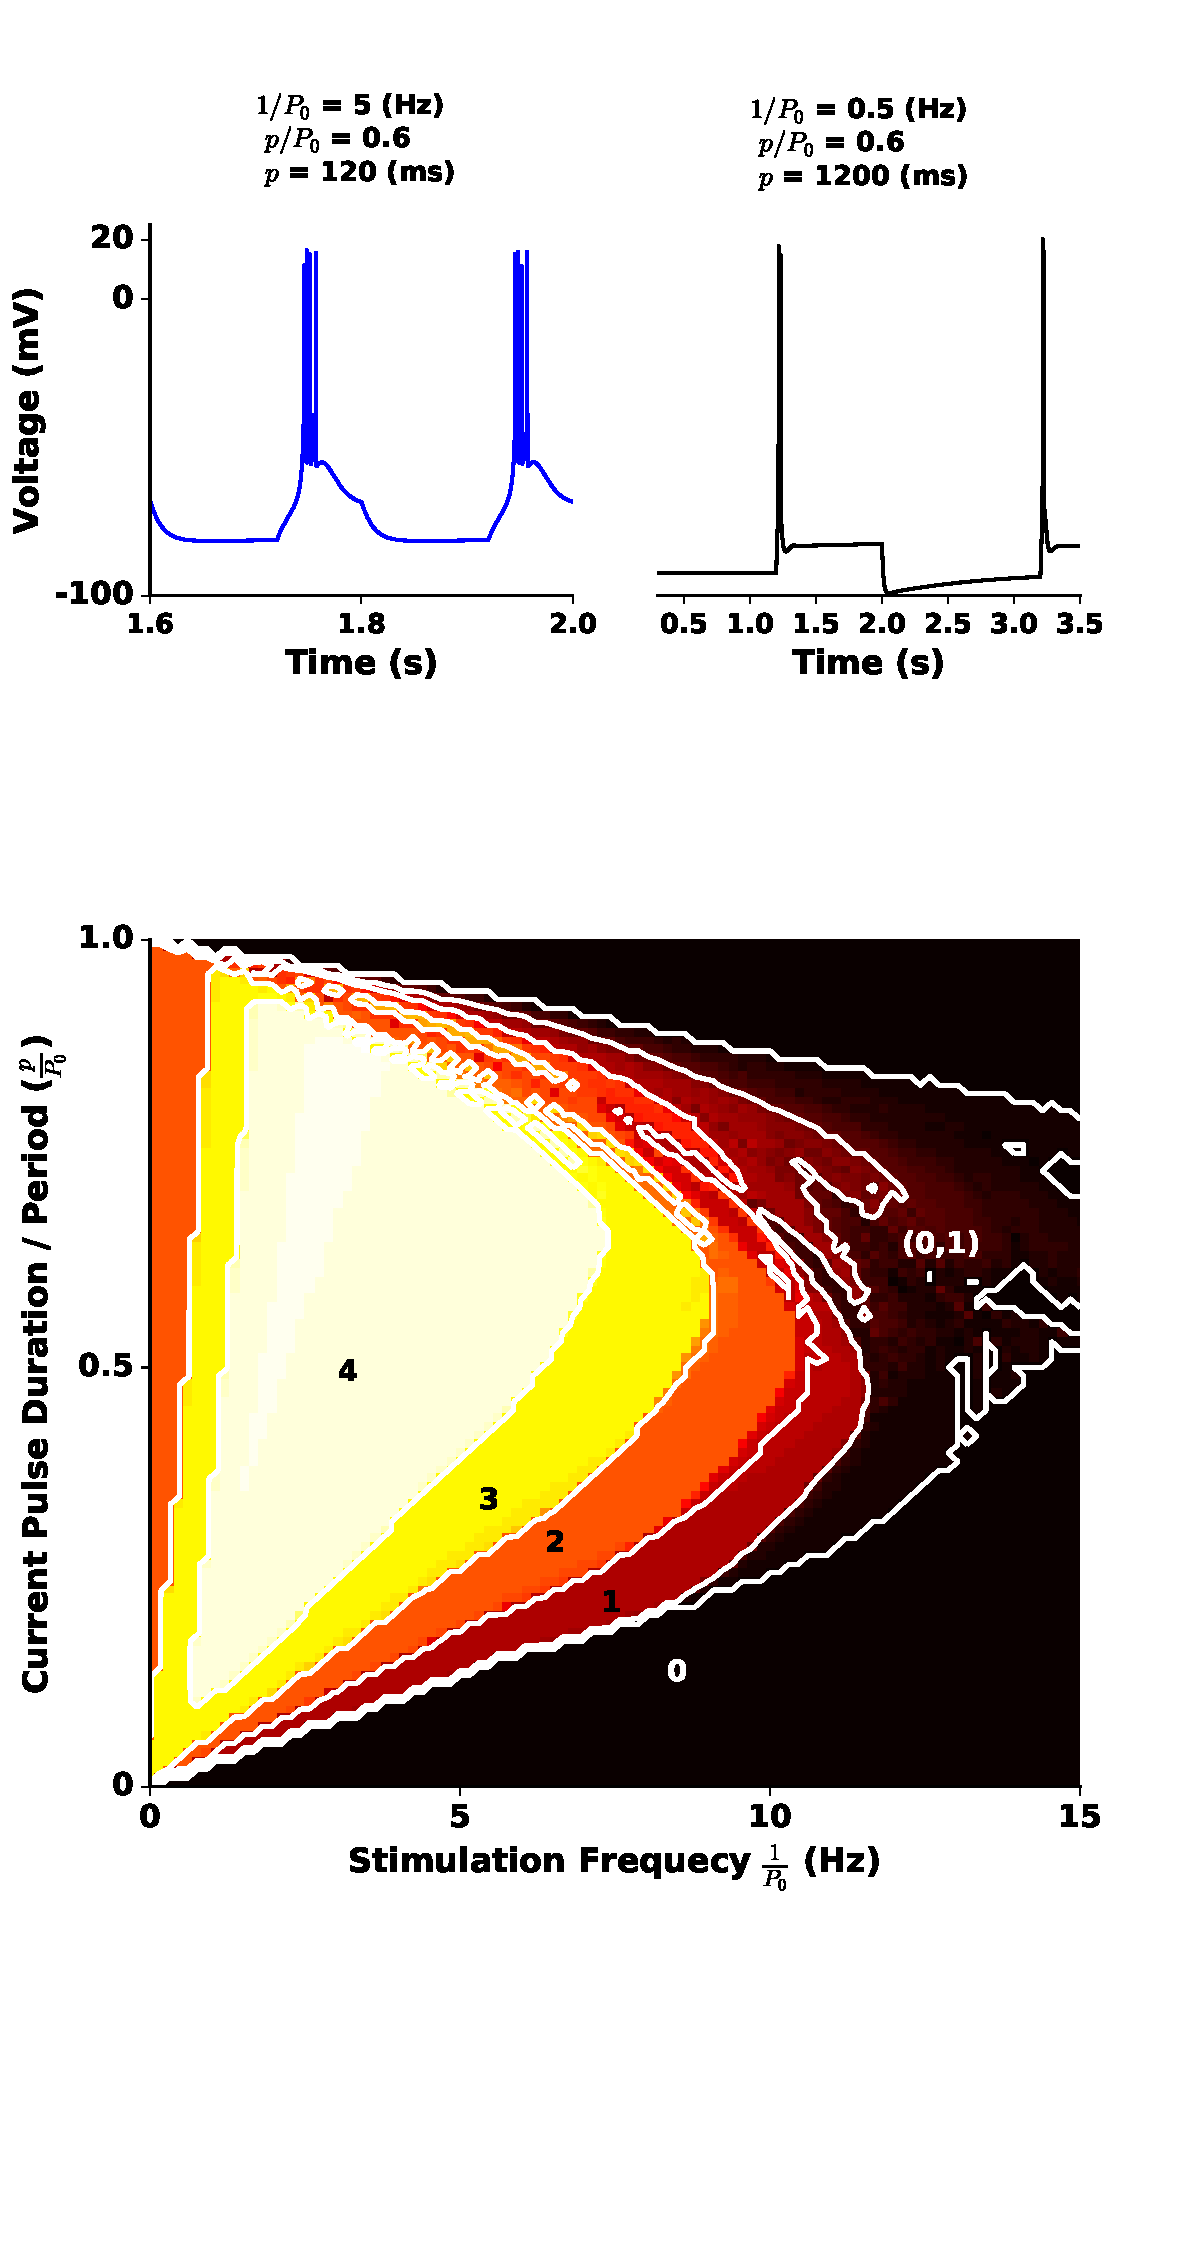
\includegraphics[width=.8\textwidth]{figs/Figure2.pdf}
    \caption{{ \bfseries \sffamily Dynamic behavior of neuron.} Here we
    simulate the model with parameters given in Table~\ref{Table:3}. The
    only parameter that changes from panel to panel in this figure is the
    external current $I_{\text{app}}$. The jet colormap indicates the different
    current values. We observe that we get quite similar results as in the original
    article \cite{wang:1994}. For instance, we obtain, repetitive spiking when
    we apply a constant current at $3 \mu A / cm^2$, or a periodic bursting 
    response, when we apply an external current of $-1.3 \mu A /cm^2$. These
    results correspond to Figure~$3$ of \cite{wang:1994}.}
    \label{Fig:2}
\end{figure}

%%
Another test case we simulated is the one that corresponds to figure $6$ of 
\cite{wang:1994}. In this test-case the neuron receives a constant
external current at $-0.95 \frac{\mu A}{cm^2}$ and as Figure~\ref{Fig:3}
points out ``spiral chaos'' is generated as in the original article.
The parameters for this simulation are given in Table~\ref{Table:4}. 
%%
\begin{figure}[!htbp]
    \centering
    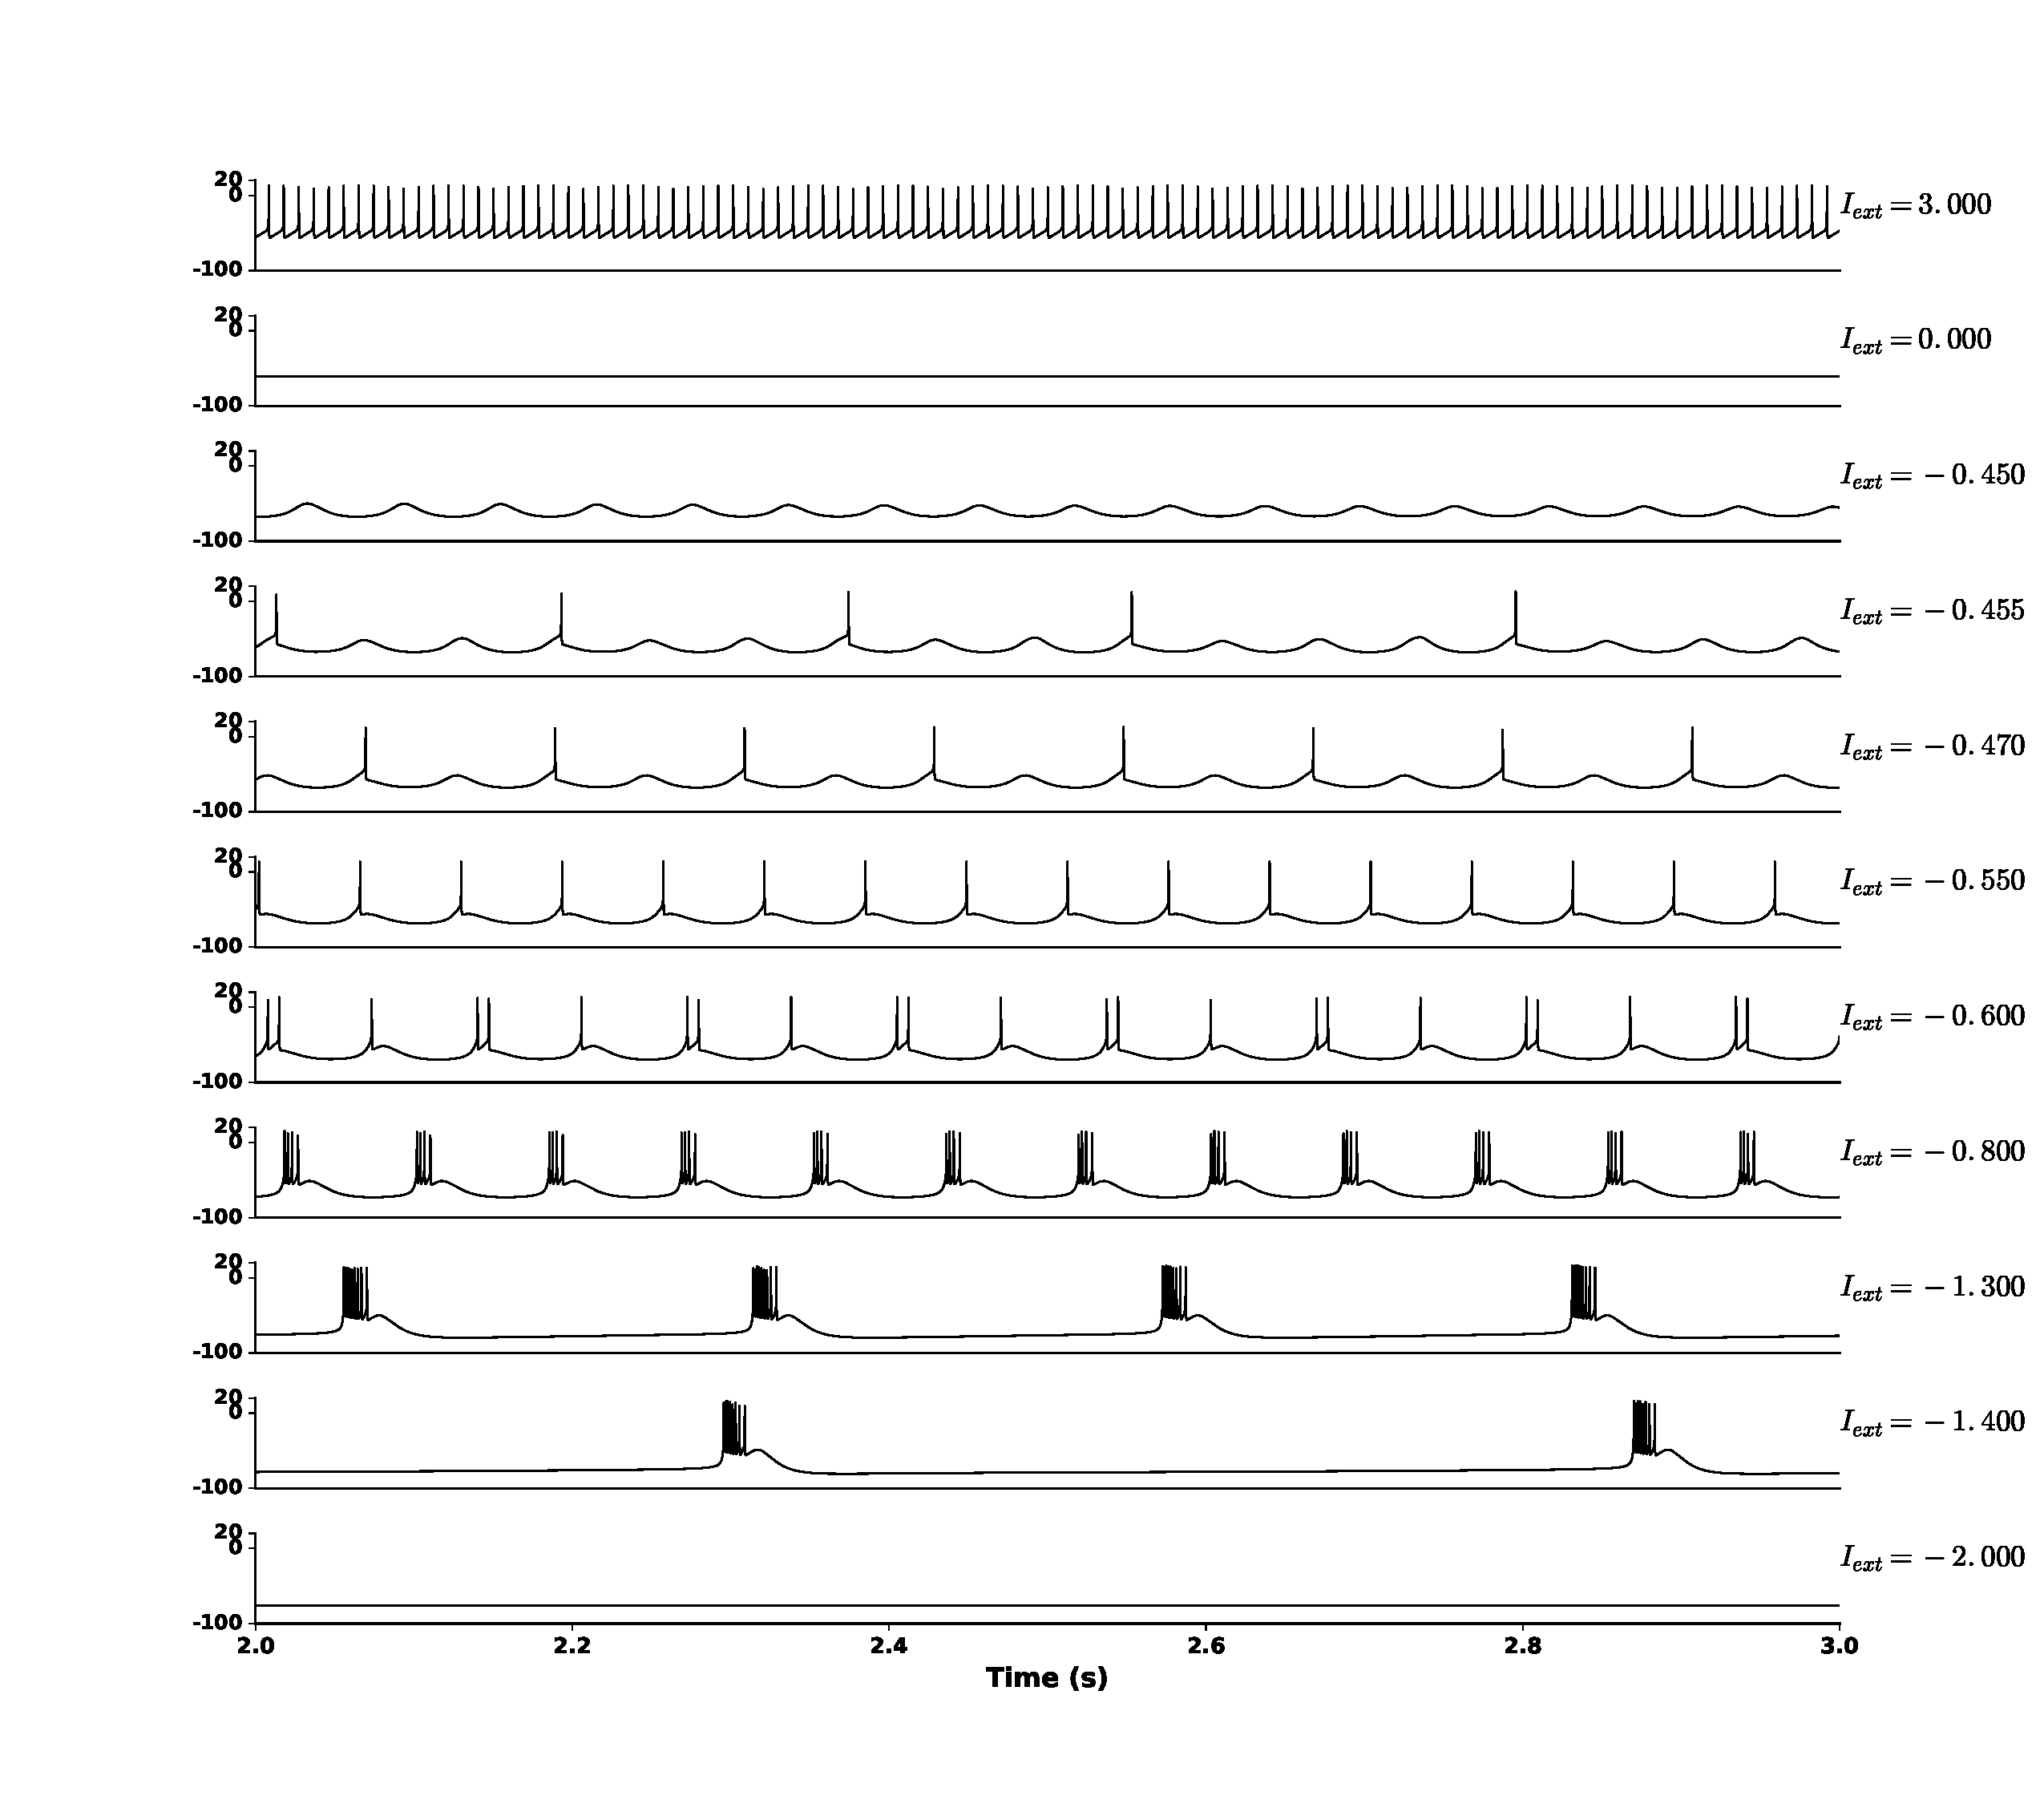
\includegraphics[width=.7\textwidth]{figs/Figure3.pdf}
    \caption{{\bfseries \sffamily ``Spiral Chaos''.} In this Figure
    we show that the model is capable of generating spiral chaos as
    it has been shown in Figure~$6$ \cite{wang:1994}. Again all the 
    parameters for this simulation are given in Table~\ref{Table:3}.
    The external current in this simulation is constant and we have 
    traced the phase portrait of the membrane potential and of the
    Sag current ($V$ vs $h$). The top panel illustrates the phase 
    portrait, the middle panel shows the membrane potential ($V$)
    and the bottom panel depicts the $h$ current over time. Our 
    results are identical to the original ones rendering 
    the model fully reproducible. }
    \label{Fig:3}
\end{figure}
%%

A fourth test case has to do with the amplitude of the injected external 
current and its relation to the frequency of the generated spike bursts. 
Therefore, we captured the data\footnote{The data are available in the
accompanying github repository of the present article.} values for the 
external current from Figure~$7$ of the original article (these are the
values represented by dots and circles in Figure $7$ and on page $27$ of
the \cite{wang:1994}) using the software
PlotDigitizer\footnote{\url{(http://plotdigitizer.sourceforge.net/})}.
Therefore, we run a simulation on the external current of the original 
article using our implementation and the results are shown in Figure 
\ref{Fig:4} upper row. Our results are pretty much the same as the ones
in Figure~$7$ of the original article. In addition, we run one more simulation
using a much higher resolution (using $200$ values of the injected current
in the range $0$ to $-2.0 \mu A/cm^2$. It is clear that the more detailed 
simulation is quantitatively similar to the simpler one but it reveals 
a more oscillatory behavior in the shape of the parameters curve. If we
superpose the two panels, we can see that the upper row is an interpolation 
of some of the data points of the bottom row.

%%
\begin{figure}[!htbp]
    \centering
    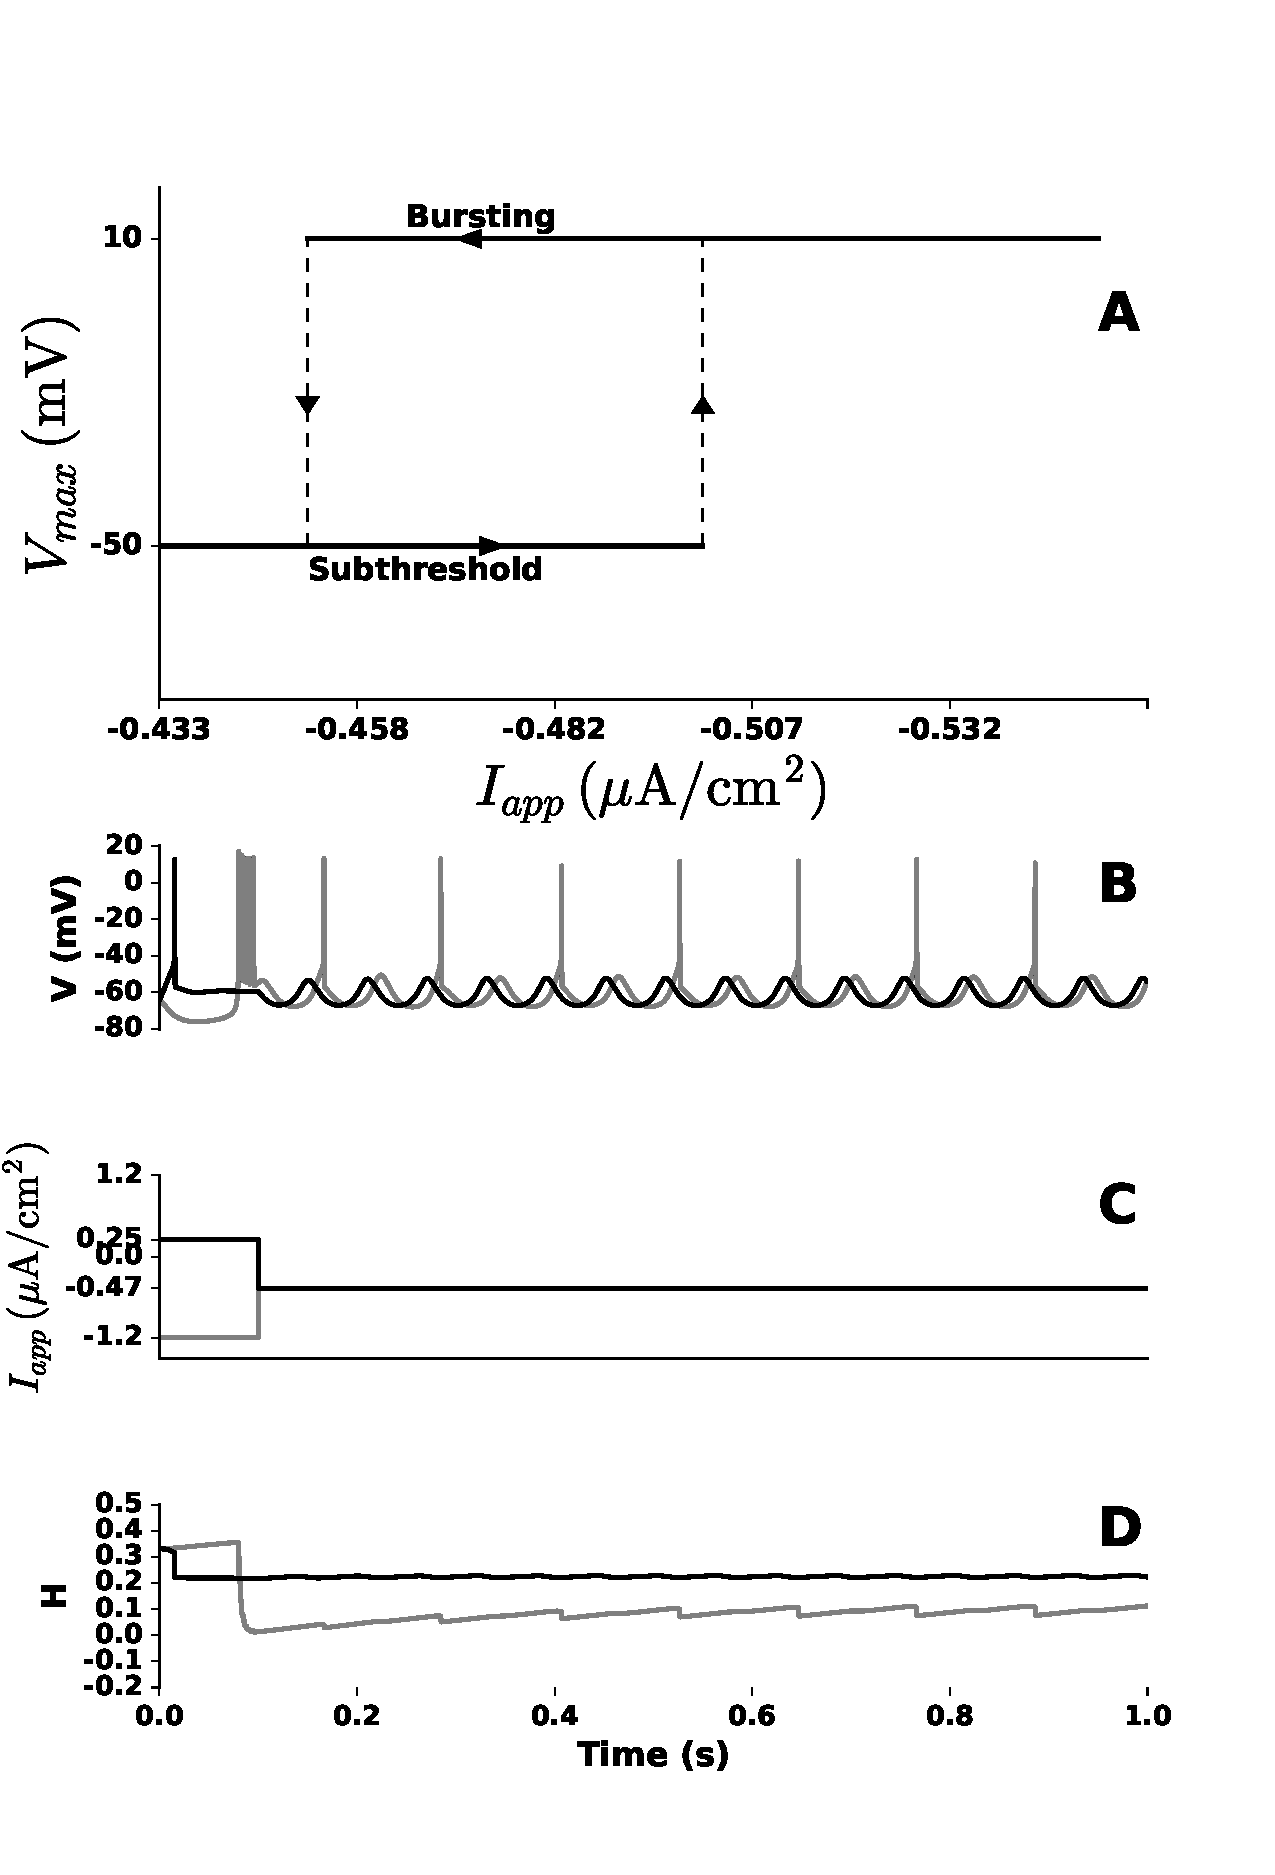
\includegraphics[width=.7\textwidth]{figs/Figure4.pdf}
    \caption{{\bfseries \sffamily Frequency and period versus steady input current.}
    {\bfseries \sffamily Top Row:} Indicates the external current (ranging from 
    $0$ to $-2 \mu A/cm^2$ versus the spike bursts frequency in $Hz$. The
    numerical values for the external current for this simulation have been
    taken from the original article (see text for more details). 
    {\bfseries \sffamily Bottom Row:} The same simulation as in the upper row,
    but with a finer discretization of the external current values range. In
    these simulations we used $200$ values for the $I_{\text{app}}$.}
    \label{Fig:4}
\end{figure}
%%

%%
\begin{figure}[!htbp]
    \centering
    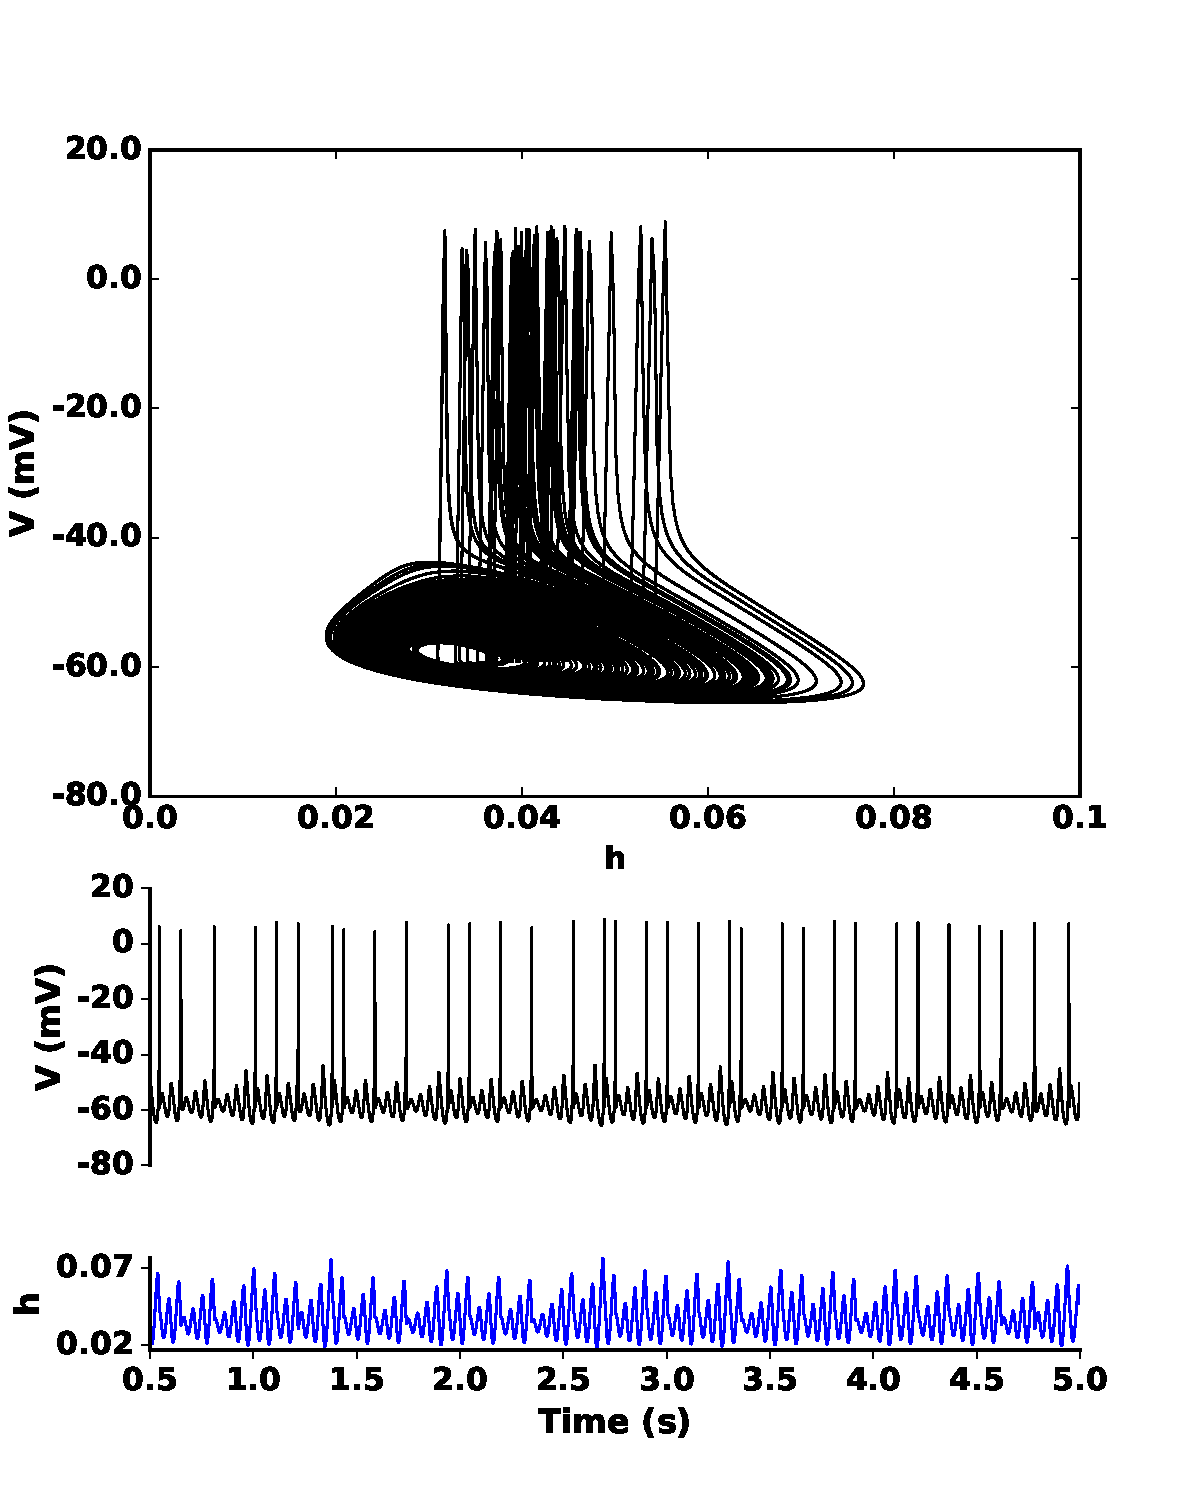
\includegraphics[width=.7\textwidth]{figs/Figure5.pdf}
    \caption{{\bfseries \sffamily Symbolic patterns.}}
    \label{Fig:5}
\end{figure}
%%

Finally, we tried to simulate some of the symbolic patterns as they are 
presented in Table~$1$ of \cite{wang:1994}. Therefore, we run our
implementation using the same parameters as in \cite{wang:1994} (see 
Table~\ref{Table:5}). The results are shown in Figure~\ref{Fig:5}, where
black dots represent zeros ($0$) and red line segments represent aces ($1$).
Different patterns emerge for different values of the external current. 
For instance, the shaded area in Figure~\ref{Fig:5} indicates that the
current is between $0.0$ and $-0.75$ and thus we have only zeros in the
formed patterns. 

\section{Conclusion}\label{conclusion}

A conductance-based model for relay thalamocortical neurons proposed 
by \cite{wang:1994} was implemented in Python. The model tested 
thoroughly in several examples taken from the original article and 
it succeed to reproduce all of them. The original model is easy to implement
since all the equations, parameters (except the initial time step of the
integration method) and simulation details are given in \cite{wang:1994}.
The choice of a different integration scheme does not affect the results,
but it increases the temporal performance of the model. 
All replicated figures are pretty much similar to the original ones rendering
the new results quantitatively and qualitatively comparable to the original
ones.

{\sffamily \small
  \printbibliography[title=References]
}
\end{document}
